\documentclass{standalone}
\usepackage{tikz}


\begin{document}

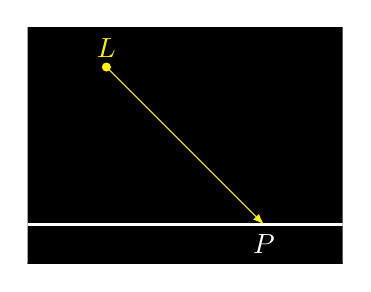
\begin{tikzpicture}
  \path[clip] (-2,-0.5) rectangle (2,2.5);
  \draw[fill=black,black] (-4,-0.5) rectangle (4,2.5);
  \draw[thick,white] (-4,0) -- (4,0);

  \coordinate (light) at (-1,2);
  \coordinate (point) at (1,0);

  \draw[yellow,fill=yellow] (light) circle [radius=0.05cm] node[above] {$L$};
  \draw[yellow,-latex] (light) -- (point);
  \node[anchor=north,white] at (point) {$P$};
\end{tikzpicture}

\end{document}